%
%   File: anteproyecto.tex
%   Author(s): Cristina Bolaños Peño
%   Copyright © 2018 Cristina Bolaños Peño
%
%   This program is free software; you can redistribute it and/or modify
%   it under the terms of the GNU General Public License as published by
%   the Free Software Foundation; either version 2 of the License, or
%   (at your option) any later version.
%
%   This program is distributed in the hope that it will be useful,
%   but WITHOUT ANY WARRANTY; without even the implied warranty of
%   MERCHANTABILITY or FITNESS FOR A PARTICULAR PURPOSE.  See the
%   GNU General Public License for more details.
%
%   You should have received a copy of the GNU General Public License
%   along with this program; if not, write to the Free Software
%   Foundation, Inc., 51 Franklin St, Fifth Floor, Boston, MA  02110-1301  USA
%

\documentclass[a4paper, 12pt, twoside]{article}

\usepackage[T1]{fontenc}
\usepackage[utf8]{inputenc}
\usepackage[spanish]{babel}
\usepackage{csquotes}
\usepackage{graphicx}
\frenchspacing
\usepackage[left=20mm, right=20mm, top=30mm, bottom=30mm, asymmetric]{geometry}
\usepackage[colorlinks=true,linkcolor=black,citecolor=black,urlcolor=black]{hyperref}
\usepackage{ragged2e}
\renewcommand{\familydefault}{\rmdefault}
\usepackage{fancyhdr}
\usepackage{titlesec}
\usepackage[backend=biber, style=apa, citestyle=apa]{biblatex}
\DeclareLanguageMapping{spanish}{spanish-apa}
\usepackage{indentfirst}

\title{Diseño de un sistema de control de riego automatizado}
\author{Cristina Bolaños Peño}
%\thanks{}

%   Page style
\renewcommand{\headrulewidth}{0pt}
\pagestyle{fancy}
\setlength{\headheight}{30pt}
\fancyhead[EL, OL]{
\includegraphics[height=0.8cm]{figures/logos/uclmRed.png}}
\fancyhead[ER, OR]{
\includegraphics[height=0.8cm]{figures/logos/esiWhite.png}}
\fancyfoot[EC, OC]{\thepage}

\newcommand{\miss}{{\bfseries\color{red}\large **}}

%   Section Style
\titleformat{\section}[block]
    {\Large\bfseries}{Capítulo \thesection}{1em}{}[]

%   Title page style
\makeatletter
\newcommand{\printDoubleRuleUpDown}{
    \par
    \rule[0.5ex]{\linewidth}{2pt}\vspace{-\baselineskip}\vspace*{3.2pt}
    \rule[0.5ex]{\linewidth}{1pt}\\[\baselineskip]
    \par
}
\newcommand{\printDoubleRuleDownUp}{
    \par
    \rule[0.5ex]{\linewidth}{1pt}\vspace{-\baselineskip}\vspace*{3.2pt}
    \rule[0.5ex]{\linewidth}{2pt}\\[\baselineskip]
    \par\vspace{6.5mm}
}
\renewcommand{\maketitle}{
    \begin{titlepage}
    \centering
    {\huge \MakeUppercase{Anteproyecto}}
    \printDoubleRuleUpDown
    {\huge \@title} \par\vspace{4mm}
    {\large\itshape Aplicado a la viticultura}
    \printDoubleRuleDownUp
    
    {\large Por} \par\vspace{6.5mm}
    {\large\scshape \@author} \par\vspace{11mm}
    
\includegraphics[scale=1]{figures/logos/departmentIcon.png} \par\vspace{6mm}
    
    {\large Departamento de Tecnologías y Sistemas de Información} \par\vspace{2mm}
    {\large\scshape Escuela Superior de Informática \par
        Universidad de Castilla-La Mancha} \par\vspace{6.5mm}
    {\large Dirigido por: Jesús Félix Villanueva Molina} \par\vspace{11mm}
    
    \justifying{Estudio sobre los factores que afectan a un cultivo y que sean medibles, a efectos de poder automatizar el riego del terreno donde se halle dicho cultivo. Así, poder conseguir unas condiciones óptimas de evolución del fruto o vegetal y garantizar la repetición estas condiciones por el medio del sistema.}
    
    \vspace{9mm}
    \centering{\large\textsc{31 de Diciembre de 2018}}
    \par\vspace{9mm}
    \small{v.1.0}
    \vspace{12mm}
    \end{titlepage}
}
\makeatother

%   Bibliography Configuration
\addbibresource{anteReferences.bib}

%   Miscellanious Configuration
\renewcommand{\labelitemi}{$\bullet$}
\renewcommand{\labelitemii}{$\diamond$}

\begin{document}

    \maketitle
    
    \renewcommand{\contentsname}{Contenido}
    \tableofcontents
    \addtocontents{toc}{\vspace{4mm} {\large Capítulo} ~\hfill\textbf{Página}\par}
%    \renewcommand{\listfigurename}{Lista de Ilustraciones}
%    \newpage \listoffigures
%    \addtocontents{lof}{\vspace{4mm} {\large Ilustración} ~\hfill\textbf{Página}\par\vspace{2mm}}
%    \renewcommand{\listtablename}{Lista de Tablas}
%    \newpage \listoftables
%    \addtocontents{lot}{\vspace{4mm} {\large Tabla} ~\hfill\textbf{Página}\par\vspace{2mm}}
    
    
\newpage
\section{Introducción}
\label{sec:Introduction}

\justifying \setlength{\parindent}{1.27cm}
\normalsize\mdseries

%   Definición del problema
El calentamiento global, la contaminación y la deforestación son conceptos plenamente conocidos y, lamentablemente, constantemente visibles en los medios de actualidad. Todos ellos afectan gravemente a las reservas de agua potable, o de uso en cultivos, del planeta, y por tanto, a la esperanza de vida humana.\newline

En Castilla-La Mancha, nuestra tierra, 7.946.198 hectáreas de terreno son dedicadas al cultivo, y sólo en 474.910 de ellas se despliegan viñedos, sin tener en cuenta las diferentes variedades de uva que los agricultores manchegos pueden o no cultivar (\cite{gob.miapa.01}). Para aprovisionar estos terrenos, se necesita un gran volumen de agua, el cual puede proceder de embalses, aguas depuradas, o acuíferos. Sin embargo, y precedida por los factores perjudiciales para el medio ambiente mencionados al inicio de este documento, la gestión de agua ante eventos extremos, por ejemplo sequías, será cada vez más importante.\newline

%   Descripciones de soluciones actuales
En la actualidad, el sector agrario emplea distintas técnicas de riego para el suministro de agua. Según el \cite{ine.01}, el agua utilizada para riego en España se despliega en las siguientes opciones:

\begin{figure}[h]
    \centering
    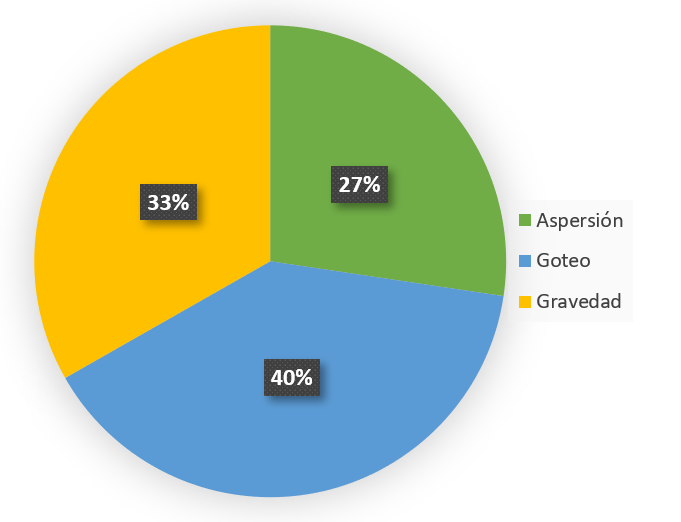
\includegraphics[scale=0.75]{figures/graphics/riego_graphic.png}
    \caption{Sistemas de riego utilizados en España.}
    \label{fig:riego_graphic}
\end{figure}

Actualmente se encuentran varias soluciones en el mercado como la aspersión, el riego por goteo o sistemas de riego automáticos dentro de invernaderos para el suministro de agua. Sin embargo, todos éstos funcionan dentro de franjas horarias sin ningún tipo de mecanismo de adaptación al terreno o a las condiciones que lo envuelven.\newline

%   Objetivos (resumen)
Es por ello que, con el fin de reducir al máximo posible el consumo de agua, con razón de cuidado de plantaciones y cultivos, se propone con este proyecto alcanzar una nueva alternativa adaptativa frente a los sistemas de riego convencionales. Para ello, se diseñará e implementará un sistema de control de riego automatizado para porciones de terreno grandes.\newline

%   Descripción de mi solución con figuras etc
La solución optada se compone de dos subsistemas diferenciados:
\begin{enumerate}
    \item Sensores y controladores del caudal del agua ({\bfseries SubLC}): Estos componentes tendrán la tarea de monitorizar los distintos factores medibles del entorno de la plantación (temperatura, humedad del suelo, etc.) y controlar el caudal necesitado por el propio terreno en función de estos.
    \item Servicio en la red ({\bfseries SubI}): Se dispondrá un servicio disponible en la red que mostrará los datos recogidos por SubLC al usuario, y además controlará al sistema SubLC.
\end{enumerate}

Se explorará más a fondo la arquitectura del sistema en el capítulo \ref{sec:target} del presente documento.
    
    
\newpage
\section{Tecnología Específica}
\label{sec:technology}
    
    
\newpage
\section{Objetivos}
\label{sec:target}
    
    
\newpage
\section{Métodos y Fases de Trabajo}
\label{sec:methods}

\justifying \setlength{\parindent}{1.27cm}
\normalsize\mdseries

Para la realización de este proyecto se empleará el Proceso Unificado de Desarrollo, en adelante referido como PUD, como metodología de planificación y trabajo. Se ha optado por dicha alternativa por su relativa sencillez, generalidad, y la amplitud de control de software que ofrece.\newline

Para diseñar y realizar los modelos de cualquier sistema, PUD hace uso del \textit{Lenguaje Unificado de Modelado} (\cite{uml.01}), en adelante referido como UML, el cual se ha utilizado en este proyecto en sus diferentes etapas. Cabe mencionar que PUD se caracteriza por estar \textbf{dirigido por casos de uso} y \textbf{centrado en la arquitectura}, mientras se trata de forma \textbf{iterativa e incremental}.\newline

Por lo tanto, y siguiendo la estructura del ciclo de vida de un producto software definido por PUD, se han establecido las siguientes pautas o fases generales a seguir:

\begin{enumerate}
    \item \textbf{Inicio}: Se llevará a cabo una descripción del producto final que se desea conseguir, estudiando el alcance del proyecto, su viabilidad, y la planificación del desarrollo del proyecto. Se obtienen:
    \begin{enumerate}
        \item Modelo de casos de uso, el cual describe las funcionalidades del sistema.
    \end{enumerate}
    \item \textbf{Elaboración}: Se desarrollará y trabajará en el modelo obtenido en la fase anterior profundizando así en la arquitectura del sistema, consiguiendo la línea base de ésta. Se obtienen:
    \begin{enumerate}
        \item Modelo de análisis, con el que desarrollamos las funcionalidades en procesos, interfaces o bancos de datos.
        \item Modelo de diseño, obteniendo un despliegue mucho más especifico del modelo anterior.
    \end{enumerate}
    \item \textbf{Construcción}: Se implementará y probará el producto, tanto su despliegue físico como el software de cada uno de sus componentes. Se obtiene:
    \begin{enumerate}
        \item Modelo de implementación, con el que se conseguirá representar la ejecución total del sistema.
        \item Modelo de pruebas, el cual contiene el conjunto de casos de pruebas unitarias que se realizan al finalizar cada una de las fases del PUD.
    \end{enumerate}
    \item \textbf{Transición}: Al llegar a esta etapa, el producto está en su versión beta y se procede a la evaluación del mismo en busca de errores o deficiencias. Se obtiene:
    \begin{enumerate}
        \item Versión del producto final.
        \item Documentación del desarrollo.
    \end{enumerate}
\end{enumerate}
    
    
\newpage
\section{Medios}
\label{sec:means}

\subsection{Medios Hardware}
\label{subsec:hardware}

Los medios hardware elegidos para desarrollar la solución aportada en este proyecto son:

\begin{itemize}
    \item \textit{Open Garden Outdoor Kit} (\cite{open.garden.01}): Se ha elegido este kit para cultivos de exteriores por la sencillez de su diseño y la gran capacidad de resolver nuestras necesidades de datos. Los componentes más relevantes del presente son:
    \begin{itemize}
        \item \textit{Open Garden Shield for Arduino} (pasarela del SubLC, en figura \ref{fig:architecture}).
        \item \textit{Open Garden Node Board} (controlador del nodo recolector en SubLC, en figura \ref{fig:architecture}).
        \item DHT22 de \textit{Open Garden} como sensor de humedad y temperatura.
        \item Sensor de humedad del terreno de \textit{Open Garden}.
    \end{itemize}
    
\end{itemize}

\subsection{Medios Software}
\label{subsec:Software}

Los medios software elegidos para desarrollar la solución aportada en este proyecto son:

\begin{itemize}
    \item MQTT (\cite{ibm.mqtt.01}): Empleado para la comunicación entre la pasarela del SubLC con los nodos de los que dispongamos.
    \item IBM Cloud (\cite{ibm.cloud.01}): Proveedor elegido para el alojamiento del subsistema SubI debido a su compromiso de colaboración con la UCLM y el acceso a sus herramientas para sus estudiantes.
    \item Flask (\cite{flask.01}): Utilizado para la creación de aplicaciones web basadas en Python (\cite{python.01}).
    \item SQL (\cite{sql.01}): Lenguaje de bases de datos utilizado para el almacenaje en el entorno \textit{cloud} de aquellos que sean pertinentes.
    \item LaTeX (\cite{latex.01}): Necesario para la realización de la memoria y del presente documento.
    \item Bitbucket (\cite{bitbucket.01}): Utilizado para el seguimiento de versiones del producto y de su documentación. Emplea Mercurial (\cite{mercurial.01}) para su uso.
    
\end{itemize}
    
%    
\newpage
\section{Contrato de Propiedad Intelectual}
\label{sec:intellectualprop}
    \newpage \section{Referencias}
    \begingroup
        \renewcommand{\section}[2]{}
        \printbibliography
    \endgroup
    
\end{document}

